\documentclass[final]{beamer}
\usepackage[size=custom,width=76.2,height=101.6,scale=1]{beamerposter}
\usepackage[T1]{fontenc}
\usepackage{lmodern,graphicx,booktabs,tikz,amsmath}
\usetikzlibrary{arrows.meta}
\setbeamertemplate{navigation symbols}{}
\setbeamertemplate{headline}{}\setbeamertemplate{footline}{}
\definecolor{ink}{HTML}{172C40}\definecolor{teal}{HTML}{007F79}
\definecolor{pale}{HTML}{EDF5F5}\definecolor{line}{HTML}{D9E2E9}
\setbeamercolor{normal text}{fg=ink,bg=white}
\newcommand{\bodyfont}{\fontsize{30}{36}\selectfont\mdseries\raggedright}
\newcommand{\smallfont}{\fontsize{27}{33}\selectfont\mdseries\raggedright}
\newcommand{\heading}[1]{{\fontsize{40}{46}\selectfont\bfseries #1}\par\vspace{0.15in}}
\newcommand{\place}[4]{\node[anchor=north west,inner sep=0,text width=#3in,align=left] at (#1,-#2) {#4};}
\begin{document}\begin{frame}[t]
\begin{tikzpicture}[remember picture,overlay,x=1in,y=1in]
\begin{scope}[shift={(current page.north west)}]
\fill[ink] (0.5,-0.5) rectangle (29.5,-4.45);
\place{1}{0.9}{28}{\color{white}\fontsize{72}{80}\selectfont\bfseries Irrelevant Features in Small-Data Tabular Learning:\\Accuracy Robustness and Runtime Costs}
\place{1}{3.15}{28}{\color{white}\fontsize{36}{42}\selectfont Arpita Shanbhag\enspace $\vert$\enspace Las Positas College}
\place{1}{3.85}{28}{\color{white!80}\fontsize{24}{29}\selectfont Stanford Data-Centric AI Workshop: Foundations, Agents, and Scientific Discovery\enspace $\vert$\enspace Nov. 3, 2026}
\fill[pale] (0.5,-4.65) rectangle (29.5,-6.25);
\place{1}{4.9}{28}{\fontsize{38}{45}\selectfont\bfseries Does predictive robustness to irrelevant features also imply low computational overhead?}
\place{1}{6.6}{28}{\heading{01\quad Matched design}}
\fill[pale] (1,-7.4) rectangle (9.6,-9.2);
\place{1.15}{7.6}{8.299999999999999}{\bodyfont\textbf{Training size}\par Five stratified 80/20 splits; nested 10\%, 50\%, 100\% training-pool subsets.}
\fill[pale] (10.5,-7.4) rectangle (19.1,-9.2);
\place{10.65}{7.6}{8.299999999999999}{\bodyfont\textbf{Feature quality}\par Clean; +50\%; +100\% independent $N(0,1)$ columns, shared across models.}
\fill[pale] (20,-7.4) rectangle (29,-9.2);
\place{20.15}{7.6}{8.7}{\bodyfont\textbf{Four fixed pipelines}\par TabPFN V2, random forest (RF), logistic regression (LR), CatBoost.}
\place{1}{9.45}{28}{\fontsize{25}{30}\selectfont\raggedright Matched examples and noise support paired comparisons. Noise precedes preprocessing; imputation and LR scaling use training data only. No tuning. One session: 1,080 configurations $\times$ 3 measured repetitions = 3,240 trials, not independent datasets.}
\place{1}{10.8}{28}{\heading{02\quad Accuracy robustness varies}}
\place{0.8}{11.85}{19.5}{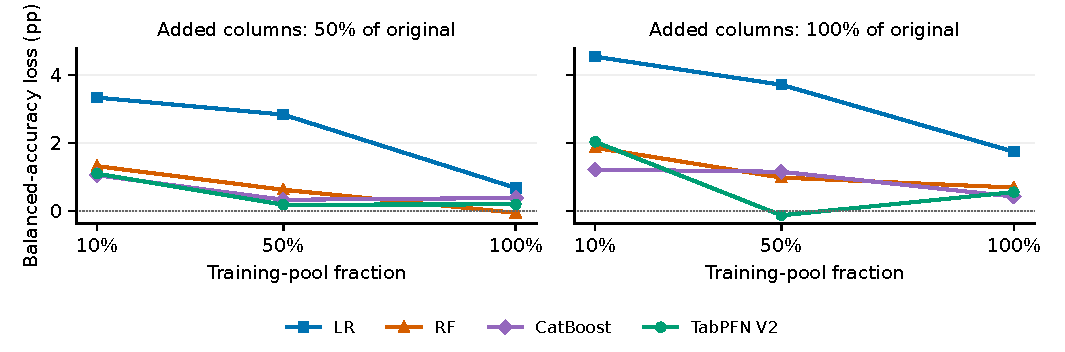
\includegraphics[width=19.5in]{figures/augmentation_loss.pdf}}
\place{21}{11.9}{8}{\bodyfont Loss = clean $-$ augmented balanced accuracy, in percentage points. Lower loss does not imply higher absolute accuracy.\par\vspace{0.25in}TabPFN's average loss is \textbf{2.15 points smaller than LR's}, 0.25 smaller than RF's, and 0.10 smaller than CatBoost's, equally weighting datasets and six conditions.\par\vspace{0.25in}\textbf{CatBoost: small, mixed difference.} Four datasets favor TabPFN; Sonar and Diabetes reverse. Contrasts range from $-0.311$ to $0.516$ points. At 10\% training/full noise, TabPFN loses 2.034 points versus 1.860 for RF and 1.217 for CatBoost.}
\place{1}{18.45}{28}{\smallfont Points average five splits within each dataset, then weight datasets equally. Negative loss denotes an observed improvement. Lines connect evaluated fractions; no population uncertainty intervals are implied.}
\draw[line,line width=1.5pt] (1,-19.55)--(29,-19.55);
\place{1}{19.85}{28}{\heading{03\quad Robustness still has a runtime cost}}
\place{0.8}{20.9}{19.5}{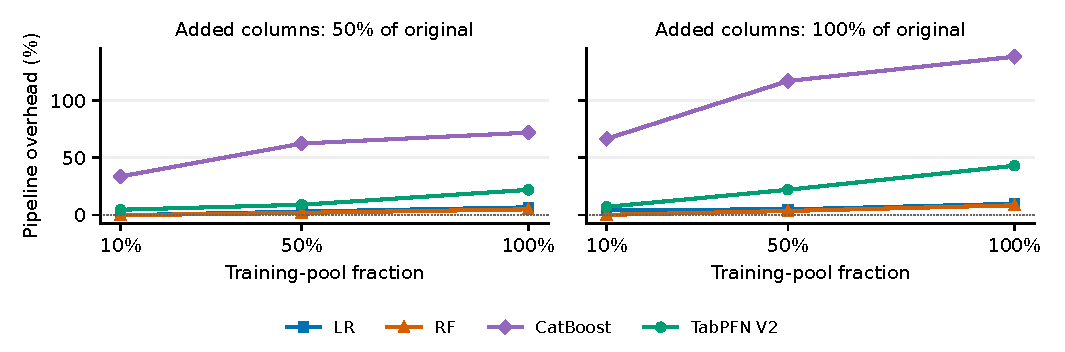
\includegraphics[width=19.5in]{figures/runtime_overhead.pdf}}
\place{21}{20.95}{8}{\bodyfont Lower overhead means a smaller relative increase, not faster execution.\par\vspace{0.25in}With full augmentation, TabPFN overhead is \textbf{7.1, 22.0, and 43.0 percent} across increasing training fractions. CatBoost's corresponding values are 66.5, 117.0, and 138.3 percent.\par\vspace{0.25in}Fit plus first prediction includes pipeline preprocessing, but excludes construction, data assembly, checkpoint download, and repeated prediction. It is not application latency. Small baseline overheads can depend on aggregation.}
\place{1}{27.5}{28}{\smallfont\textbf{TabPFN: Tesla T4 GPU. All baselines: CPU.} Median paired ratios over three repetitions, then equal means over splits and datasets. Warm-ups, randomized order, and CUDA synchronization support timing comparisons.}
\draw[line,line width=1.5pt] (1,-28.7)--(29,-28.7);
\place{1}{29.05}{13.4}{\heading{04\quad Fitting and prediction differ}\fontsize{30}{36}\selectfont\raggedright Half training/full noise, a secondary condition selected after inspecting accuracy. Times are equal-dataset means of per-split medians, in milliseconds.\par\vspace{0.16in}
{\fontsize{34}{41}\selectfont\renewcommand{\arraystretch}{1.45}\setlength{\tabcolsep}{16pt}\begin{tabular}{lrrr}\toprule
 & Fit & First batch & Second batch\\\midrule
CatBoost (CPU) & 2813.69 & 1.61 & 1.35\\
TabPFN V2 (GPU) & 83.05 & 155.73 & 155.90\\\bottomrule
\end{tabular}}\par\vspace{0.18in}\smallfont CatBoost's larger combined cost is dominated by fitting. Its batch prediction is faster here. These are not per-example latencies or a hardware-neutral serving benchmark.}
\place{15.6}{29.05}{13.4}{\heading{05\quad Scope and practical implication}\fontsize{34}{41}\selectfont\raggedright Six convenience-selected tasks: Iris, Wine, Breast Cancer, Sonar, Ionosphere, and Diabetes; 12--614 training examples. Fixed configurations, Gaussian distractors, exploratory accuracy comparisons, and one timing environment constrain generalization.\par\vspace{0.18in}Repeated splits and nested subsets are dependent. We do not establish significance, equivalence, feature-selection savings, or energy savings. Noisy features known by construction differ from unknown distractors in deployed data.}
\fill[pale] (0.5,-35.65) rectangle (29.5,-37.45);
\place{1}{35.9}{28}{\fontsize{29}{36}\selectfont\bfseries\color{teal}Small accuracy losses can coexist with increased computational cost. Evaluate absolute accuracy, robustness to irrelevant features, and fitting and prediction times separately across training sizes and feature-quality conditions.}
\place{1}{37.7}{18.5}{\fontsize{19}{23}\selectfont\textbf{Selected context}\quad Hollmann et al., \emph{Nature} 637, 319--326 (2025), doi:10.1038/s41586-024-08328-6.\par Hu and Ghelichi, \emph{Noise Immunity in In-Context Tabular Learning}, arXiv:2604.04868v2 (2026).\par Feuer, Hegde, and Cohen, \emph{Scaling TabPFN}, arXiv:2311.10609 (2023).}
\end{scope}\end{tikzpicture}\end{frame}\end{document}
